\documentclass{beamer}
\mode<presentation>
\usepackage{amsmath}
\usepackage{amssymb}
%\usepackage{advdate}
\usepackage{adjustbox}
\usepackage{subcaption}
\usepackage{enumitem}
\usepackage{multicol}
\usepackage{mathtools}
\usepackage{listings}
\usepackage{url}
\usepackage{tikz}
\usetikzlibrary{matrix}
\def\UrlBreaks{\do\/\do-}
\usetheme{metropolis}
%\usecolortheme{lily}
\setbeamertemplate{footline}
{
  \leavevmode%
  \hbox{%
  \begin{beamercolorbox}[wd=\paperwidth,ht=2.25ex,dp=1ex,right]{author in head/foot}%
    \insertframenumber{} / \inserttotalframenumber\hspace*{2ex} 
  \end{beamercolorbox}}%
  \vskip0pt%
}
\setbeamertemplate{navigation symbols}{}

\providecommand{\nCr}[2]{\,^{#1}C_{#2}} % nCr
\providecommand{\nPr}[2]{\,^{#1}P_{#2}} % nPr
\providecommand{\mbf}{\mathbf}
\providecommand{\pr}[1]{\ensuremath{\Pr\left(#1\right)}}
\providecommand{\qfunc}[1]{\ensuremath{Q\left(#1\right)}}
\providecommand{\sbrak}[1]{\ensuremath{{}\left[#1\right]}}
\providecommand{\lsbrak}[1]{\ensuremath{{}\left[#1\right.}}
\providecommand{\rsbrak}[1]{\ensuremath{{}\left.#1\right]}}
\providecommand{\brak}[1]{\ensuremath{\left(#1\right)}}
\providecommand{\lbrak}[1]{\ensuremath{\left(#1\right.}}
\providecommand{\rbrak}[1]{\ensuremath{\left.#1\right)}}
\providecommand{\cbrak}[1]{\ensuremath{\left\{#1\right\}}}
\providecommand{\lcbrak}[1]{\ensuremath{\left\{#1\right.}}
\providecommand{\rcbrak}[1]{\ensuremath{\left.#1\right\}}}
\theoremstyle{remark}
\newtheorem{rem}{Remark}
\newcommand{\sgn}{\mathop{\mathrm{sgn}}}
\providecommand{\abs}[1]{\left\vert#1\right\vert}
\providecommand{\res}[1]{\Res\displaylimits_{#1}} 
\providecommand{\norm}[1]{\lVert#1\rVert}
\providecommand{\mtx}[1]{\mathbf{#1}}
\providecommand{\mean}[1]{E\left[ #1 \right]}
\providecommand{\fourier}{\overset{\mathcal{F}}{ \rightleftharpoons}}
%\providecommand{\hilbert}{\overset{\mathcal{H}}{ \rightleftharpoons}}
\providecommand{\system}{\overset{\mathcal{H}}{ \longleftrightarrow}}
	%\newcommand{\solution}[2]{\textbf{Solution:}{#1}}
%\newcommand{\solution}{\noindent \textbf{Solution: }}
\providecommand{\dec}[2]{\ensuremath{\overset{#1}{\underset{#2}{\gtrless}}}}
\newcommand{\myvec}[1]{\ensuremath{\begin{pmatrix}#1\end{pmatrix}}}
\let\vec\mathbf

\lstset{
%language=C,
frame=single, 
breaklines=true,
columns=fullflexible
}

\numberwithin{equation}{section}

\title{Computationally solving quadratic equations \brak{\text{10.4.2.6}}}
\author{Agamjot Singh,\\EE24BTECH11002,\\IIT Hyderabad.}

\date{\today} 
\begin{document}

\begin{frame}
\titlepage
\end{frame}

\section*{Outline}
\begin{frame}
\frametitle{Table of Contents}
\tableofcontents
\end{frame}

\section{Problem}

\begin{frame}
\frametitle{Problem Statement}
A cottage industry produces a certain number of pottery articles in a day. It was observed on a particular day that the cost of production of each article \brak{\text{in rupees}} was $3$ more than twice the number of articles produced on that day. If the total cost of production on that day was $90$, find the number of articles produced and the cost of each article.
\end{frame}

\section{Solution}

%Slide1
\subsection{Theoretical Solution}
\begin{frame}
\frametitle{Theoretical Solution}
Let the number of articles produced in a day be $x$, then the above question can the following quadratic equation will be formed.
\begin{align}
  \brak{3 + 2x}x &= 90\\
  2x^2 + 3x - 90 &= 0
\end{align}
Theoretically, it can easily be solved using the quadratic formula,
\begin{align}
  x = \frac{-3 \pm \sqrt{729}}{4} = 6, -7.5
\end{align}
\end{frame}

%Slide2
\subsection{Computation Solution - Newton Raphson's Method}
\begin{frame}
\frametitle{Computation Solution - Newton Raphson's Method}
Now we use the \textbf{Newton-Raphson method} to computationally find the roots.
\newline
Let 
\begin{align}
  f\brak{x} &= 2x^2 + 3x - 90\\
  \implies f^{\prime}\brak{x} &= 4x + 3
\end{align}
The difference equation by the Newton-Raphson method is given by,
\begin{align}
  x_{n + 1} = x_n - \frac{f\brak{x_n}}{f^{\prime}\brak{x_n}} \text{, } f^{\prime}\brak{x_n} \neq 0
\end{align}
If we, at any point, encouter a situation in which $f^{\prime}\brak{x_n} = 0$, it implies that our inital guess leads to failure of the Newton method to converge to a root and we have to abandon and restart with another intial guess.
\end{frame}

%Slide3
\begin{frame}
Substituting $f\brak{x}$ and $f^{\prime}\brak{x}$ in the difference equation, we get,
\begin{align}
  x_{n + 1} &= x_n - \brak{\frac{2\brak{x_n}^2 + 3x_n - 90}{4x_n + 3}}\\
  x_{n + 1} &= \frac{2\brak{x_n}^2 + 90}{4x_n + 3} \text{, } x_n \neq -\frac{3}{4}
\end{align}
Taking initial guess $\brak{x_0} = 8$, we get the root as $x = 6.000000476837158$.
Taking initial guess $\brak{x_0} = -8$, we get the root as $x = -7.500000476837158$.
\end{frame}

%Slide4
\subsection{Computation Solution - Eigenvalue Method}
\begin{frame}
\frametitle{Computation Solution - Eigenvalue Method}
Frobenius \textbf{companion matrix} for a polynomial $p$ of the form,
\begin{align}
  p\brak{x} = c_0 + c_1x + c_2x^2 + \dots + c_{n - 1}x^{n - 1} + x^n
\end{align}
is given by
\begin{align}
  C\brak{p} = \myvec{0 & 0 & \dots & 0 & -c_0\\1 & 0 & \dots & 0 & -c_1\\0 & 1 & \dots & 0 & -c_2\\\vdots & \vdots & \ddots & \vdots & \vdots\\0 & 0 & \dots & 1 & -c_{n - 1}}
\end{align}
\end{frame}

%Slide6
\begin{frame}
The eigen values of this companion matrix are the roots of the polynomial $p$. This is because of the characteristic polynomial for this matrix being
\begin{align}
  c_0I + c_1C + c_2C^2 + \dots + c_{n - 1}C^{n - 1} + C^n &= 0\\
  c_0 + c_1\lambda + c_2\lambda^2 + \dots + c_{n - 1}\lambda^{n - 1} + \lambda^n &= 0\\
\end{align}
where $\lambda$ is the eigenvalue of $C\brak{p}$.
\begin{align}
    p\brak{x} &= x^2 + \frac{3}{2}x - 45 = 0\\
    C\brak{p} &= \myvec{0 & 45\\1 & -1.5}
\end{align}
\end{frame}

%Slide7
\begin{frame}
We find the eigenvalues using the $QR$ algorithm. The basic principle behind this algorithm is a similarity transform,
\begin{align}
  A^{\prime} = X^{-1}AX
\end{align}
which does not alter the eigenvalues of the matrix A. 
\newline
We use this to get the Schur Decomposition,
\begin{align}
  A = Q^{-1}UQ = Q^{\ast}UQ
\end{align}
where $Q$ is a unitary matrix $\brak{Q^{-1} = Q^{\ast}}$ and $U$ is an upper triangular matrix whose diagonal entries are the eigenvalues of $A$.
\newline
To efficiently get the Schur Decomposition, we first householder reflections to reduce it to an upper hessenberg form.
\end{frame}

%Slide8
\begin{frame}
A householder reflector matrix is of the form,
\begin{align}
  P = I - 2\vec{u}\vec{u^{\ast}}
\end{align}
Householder reflectors transforms any vector $\vec{x}$ to a multiple of $\vec{e_1}$,
\begin{align}
  P\vec{x} = \vec{x} - 2\vec{u}\brak{\vec{u^{\ast}}\vec{x}} = \alpha \vec{e_1}
\end{align}
P is unitary, which implies that,
\begin{align}
  \norm{P\vec{x}} &= \norm{\vec{x}}\\
  \implies \alpha &= \rho\norm{\vec{x}}\\
\end{align}
\end{frame}

%Slide9
\begin{frame}
As $\vec{u}$ is unit norm,
\begin{align}
  \vec{u} = \frac{\vec{x} - \rho\norm{\vec{x}}\vec{e_1}}{\norm{\vec{x} - \rho\norm{\vec{x}}\vec{e_1}}} = \frac{1}{\norm{\vec{x} - \rho\norm{\vec{x}}\vec{e_1}}} \begin{pmatrix} x_1 - \rho\norm{\vec{x}}\\x_2\\\vdots\\x_n\end{pmatrix}
\end{align}
Selection of $\rho$ is flexible as long as $\abs{\rho} = 1$. To ease out the process, we take $\rho = \frac{x_1}{\abs{x_1}}$, $x_1 \neq 0$. If $x_1 = 0$, we take $\rho = 1$.
\newline
Householder reflector matrix $\brak{P_{i}}$ is given by,
\begin{align}
  P_{i} = \begin{bmatrix}
    1 & 0 & 0 & 0 & 0\\    
    0 & \times & \times & \times & \times\\
    0 & \times & \times & \times & \times\\
    0 & \times & \times & \times & \times\\
    0 & \times & \times & \times & \times
  \end{bmatrix} = \begin{bmatrix}
    1 & \vec{0}^{\ast}\\    
    \vec{0} & I_{n - i} - 2\vec{u_{i}}\vec{u_{i}^{\ast}}
  \end{bmatrix}
\end{align}
\end{frame}

%Slide10
\begin{frame}
\begin{align}
A = 
\begin{bmatrix}
\times & \times & \times & \times \\
\times & \times & \times & \times \\
\times & \times & \times & \times \\
\times & \times & \times & \times
\end{bmatrix}
\xrightarrow{P_1}
\begin{bmatrix}
\times & \times & \times & \times \\
\times & \times & \times & \times \\
0 & \times & \times & \times \\
0 & \times & \times & \times
\end{bmatrix}
\xrightarrow{P_2}
\begin{bmatrix}
\times & \times & \times & \times \\
\times & \times & \times & \times \\
0 & \times & \times & \times \\
0 & 0 & \times & \times
\end{bmatrix}
\end{align}
Next step is to do Given's rotation to get the $QR$ Decomposition.
\end{frame}

%Slide11
\begin{frame}
The Givens rotation matrix $G\brak{i, j, c, s}$ is defined by
\begin{align}
G\brak{i, j, c, s} = \begin{bmatrix}
1 & \cdots & 0 & \cdots & 0 & \cdots & 0 \\
\vdots & \ddots & \vdots & \ddots & \vdots & \ddots & \vdots \\
0 & \cdots & c & \cdots & s & \cdots & 0 \\
\vdots & \ddots & \vdots & \ddots & \vdots & \ddots & \vdots \\
0 & \cdots & -\overline{s} & \cdots & \overline{c} & \cdots & 0 \\
\vdots & \ddots & \vdots & \ddots & \vdots & \ddots & \vdots \\
0 & \cdots & 0 & \cdots & 0 & \cdots & 1
\end{bmatrix}
\end{align}
where $\abs{c}^2 + \abs{s}^2 = 1$, and $G$ is a unitary matrix.
\end{frame}

%Slide
\begin{frame}
Say we take a vector $\vec{x}$, and $\vec{y} = G\brak{i, j, c, s}\vec{x}$, then
\begin{align}
    y_k = \begin{cases}
        c x_i + s x_j, & k = i \\
        -\overline{s} x_i + \overline{c} x_j, & k = j \\
        x_k, & k \neq i, j
    \end{cases}
\end{align}
For $y_j$ to be zero, we set
\begin{align}
    c = \frac{\overline{x_i}}{\sqrt{\abs{x_i}^2 + \abs{x_j}^2}} = c_{ij}\\
    s = \frac{\overline{x_j}}{\sqrt{\abs{x_i}^2 + \abs{x_j}^2}} = s_{ij}
\end{align}
Using this Givens rotation matrix, we zero out elements of subdiagonal in the hessenberg matrix $H$.
\end{frame}

%Slide
\begin{frame}

\begin{multline}
H = \begin{bmatrix}
\times & \times & \times & \times & \times\\
\times & \times & \times & \times & \times\\
0 & \times & \times & \times & \times\\
0 & 0 & \times & \times & \times\\
0 & 0 & 0 & \times & \times
\end{bmatrix} \xrightarrow{G\brak{1, 2, c_{12}, s_{12}}}
\begin{bmatrix}
\times & \times & \times & \times & \times\\
0 & \times & \times & \times & \times\\
0 & \times & \times & \times & \times\\
0 & 0 & \times & \times & \times\\
0 & 0 & 0 & \times & \times
\end{bmatrix} \\\xrightarrow{G\brak{2, 3, c_{23}, s_{23}}}
\begin{bmatrix}
\times & \times & \times & \times & \times\\
0 & \times & \times & \times & \times\\
0 & 0 & \times & \times & \times\\
0 & 0 & \times & \times & \times\\
0 & 0 & 0 & \times & \times
\end{bmatrix} \xrightarrow{G\brak{3, 4, c_{34}, s_{34}}}
\begin{bmatrix}
\times & \times & \times & \times & \times\\
0 & \times & \times & \times & \times\\
0 & 0 & \times & \times & \times\\
0 & 0 & 0 & \times & \times\\
0 & 0 & 0 & \times & \times
\end{bmatrix} \\\xrightarrow{G\brak{4, 5, c_{45}, s_{45}}}
\begin{bmatrix}
\times & \times & \times & \times & \times\\
0 & \times & \times & \times & \times\\
0 & 0 & \times & \times & \times\\
0 & 0 & 0 & \times & \times\\
0 & 0 & 0 & 0 & \times
\end{bmatrix} = R
\end{multline}
\end{frame}

%Slide
\begin{frame}
where $R$ is upper triangular.
\newline
For the given companion matrix,
\begin{align}
  c_{11} = \frac{0}{\sqrt{0^2 + 1^2}} = 0\\
  s_{11} = \frac{1}{\sqrt{0^2 + 1^2}} = 1
\end{align}
Let $G_k = G\brak{k, k + 1, c_{k, k+1}, s_{k, k+1}}$, then we deduce that
\begin{align}
    G_4 G_3 G_2 G_1 H &= R\\
    H &= G_1^{\ast} G_2^{\ast} G_3^{\ast} G_4^{\ast} R\\
    H &= QR, \text{ where } Q = G_1^{\ast} G_2^{\ast} G_3^{\ast} G_4^{\ast}
\end{align}
Using this $QR$ algorithm, we get the following update equation,
\begin{align}
  A_{k} &= Q_{k}R_{k}\\
  A_{k + 1} &= R_{k}Q_{k}\\
            &= \brak{G_{n}\dots G_{2} G_{1}} A_{k} \brak{G_1^{\ast} G_2^{\ast} \dots G_n^{\ast}}
\end{align}
\end{frame}

\begin{frame}
    The $QR$ algorithm will sometimes converge to matrix which is of the form where some subdiagonal elements will not converge to 0, and there will be $2\times2$ blocks protruding the diagonal of the matrix. 
    These can be solved be taking all such blocks, and then taking the eigenvalues of all these sub $2\times 2$ matrix blocks.
    \newline
    \newline
    Running the eigenvalue code for our companion matrix we get,
    \begin{align}
        6 + 0.0i, -7.5 + 0.0i
    \end{align}
\end{frame}

%Slide12
\subsection{Plot}
\begin{frame}
\frametitle{Plot}
\begin{figure}[h!]
   \centering
   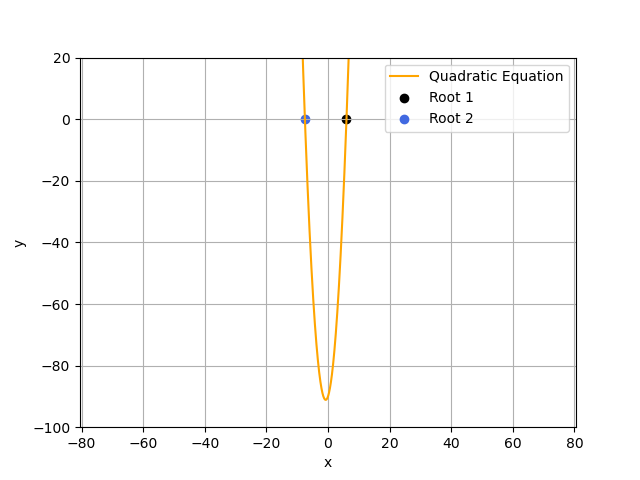
\includegraphics[width=0.7\linewidth]{figs/graph.png}
   \caption{Objective Function with the minimum point}
\end{figure}
\end{frame}

\end{document}
